\title{\Large \textbf{Modelling the Age of Abalone}}
\author{\small 450132759}
\date{\small October 29, 2018}

\documentclass[9pt,twocolumn]{article}
%\usepackage{fullpage} % full parge margins
\usepackage[margin=0.5in]{geometry}
\usepackage{hyperref} % allows for linking urls
\usepackage[superscript,biblabel]{cite} % superscript while citing
\usepackage{booktabs}
\usepackage{graphicx} % allows for adding figures
\usepackage{subcaption} % allows for adding subfigures
\usepackage{enumitem} % allows for lists
\usepackage{amsmath} % allows for math equations
\usepackage{gensymb} % degree symbol, usage: \degree
\usepackage{csvsimple}
\usepackage{booktabs} % to generate booktabs style tables
\usepackage{lscape}
\usepackage{siunitx}
\usepackage{tikz} % To generate the plot from csv
\usepackage{pgfplots}
\pgfplotsset{compat=newest} % Allows to place the legend below plot
\usepackage{placeins} % Use in conjunction with \FloatBarrier to limit floating of figures
\usepackage{sectsty} % allows for defining section styles
\sectionfont{\fontsize{12}{13}\selectfont} % defines font size of sections

\begin{document}
	\begin{center}
		\textbf{\Large Modelling the Age of Abalone} \\\vspace{4mm}
		\texttt{450132759 / 450237777\\470315518 / 470396894}
	\end{center}
	\begin{abstract}
		The Blacklip Abalone, scientific name Haliotis rubra, is common to several parts of Australia \cite{source}. They are fished recreationally and also farmed. A data set provided by University of California Irvine, originally from the Department of Primary Industry and Fisheries, Tasmania, consists of several physical characteristics, including the number of rings of the Blacklip Abalone shell. The number of rings acts as proxy for the age of the Abalone. We set out to determine and compare both the best and most practical model of age of the abalone using multiple regression. This could then be used to develop and enforce recreational fishing regulations and also to maintain helathy farmed populations. Beginning with a full model, we employ step backward model selection using the Akaike information criterion (AIC). This is compared with a step forward AIC and also a practical model using easy to measure explantory variables. The practical model first removes highly correlated variables using a test for multicollinearity. We then remove difficult to measure explantory variables and test the performance of the resultant model. Our analysis finds that a practical model performs well compared to the stepwise model and can form the basis for developing best harvesting practices both recreationally and for the Blacklip Abalone Farming industry.
	\end{abstract}

	\section{Introduction}
		Abalone meat is used as a food delicacy, its shells are a foundation for certain types of jewellery and it functions ecologically to stablize kelp forrests and algae in its rocky reef habitat. Blacklip Abalone reach sexual maturity after three to six years and spawning occurs between Spring and Autumn\cite{blacklip}. Given the importance of a healthy Abalone population, both in the wild and when farmed, it is crucial to develop, apply and regulate best harvesting practices to maintain healthy Abalone populations. With this in mind, we question how well an unrestriced model using all explanatory variables predicts the age of the Blacklip Abalone. An attempt is then made to build a practical model that can be deployed by farmers and regulators allike that provides a similar level of predictive power but doesn't necessitate killing the Abalone or require the use of specialized equipment.					
	\section{Data Set}
	
		The data is provided by the Machine Leanring Repository at University of California Irvine. It was orginally obtained from the Department of Primary Industry and Fisheries, Tasmania. The variables are:
		\begin{table}[!htbp]
			\resizebox{\columnwidth}{!}{%
				\begin{tabular}{@{}llll@{}}
					\toprule
					Variable        & Type       & Dimension & Description                 \\ \midrule
					Sex             & nominal    &           & M, F and I (infant)         \\
					Length          & continuous & mm        & Longest shell measurement   \\
					Diameter        & continuous & mm        & perpendicular to length     \\
					Height          & continuous & mm        & with meat in shell          \\
					Whole\_weight   & continuous & g         & whole abalone               \\
					Shucked\_weight & continuous & g         & weight of meat              \\
					Viscera\_weight & continuous & g         & gut weight (after bleeding) \\
					Shell\_weight   & continuous & g         & after being dried           \\
					Rings           & integer    &           & + 1.5 gives age in years    \\ \bottomrule
				\end{tabular}%
			}
			\caption{Description of Data Set}
		\end{table}	
		
		After assigning new variable names to each column, we checked the assumption for multicollinearity. Linear regression assumes that there is little or no multicollinearity in the data; however, from the ggpairs output, most of the variables were relatively highly correlated with one another. The variables with few of the highest correlations were between length and diameter, as well as whole weight and the other weight predictors. Moreover, we found out that despite the difference in their means, male and female seemed to have similar distributions. So from such results, we decided to combine male and female into one category along with removing either length, or diameter from the model.
		
		\begin{figure}[!htbp]
			\centering
			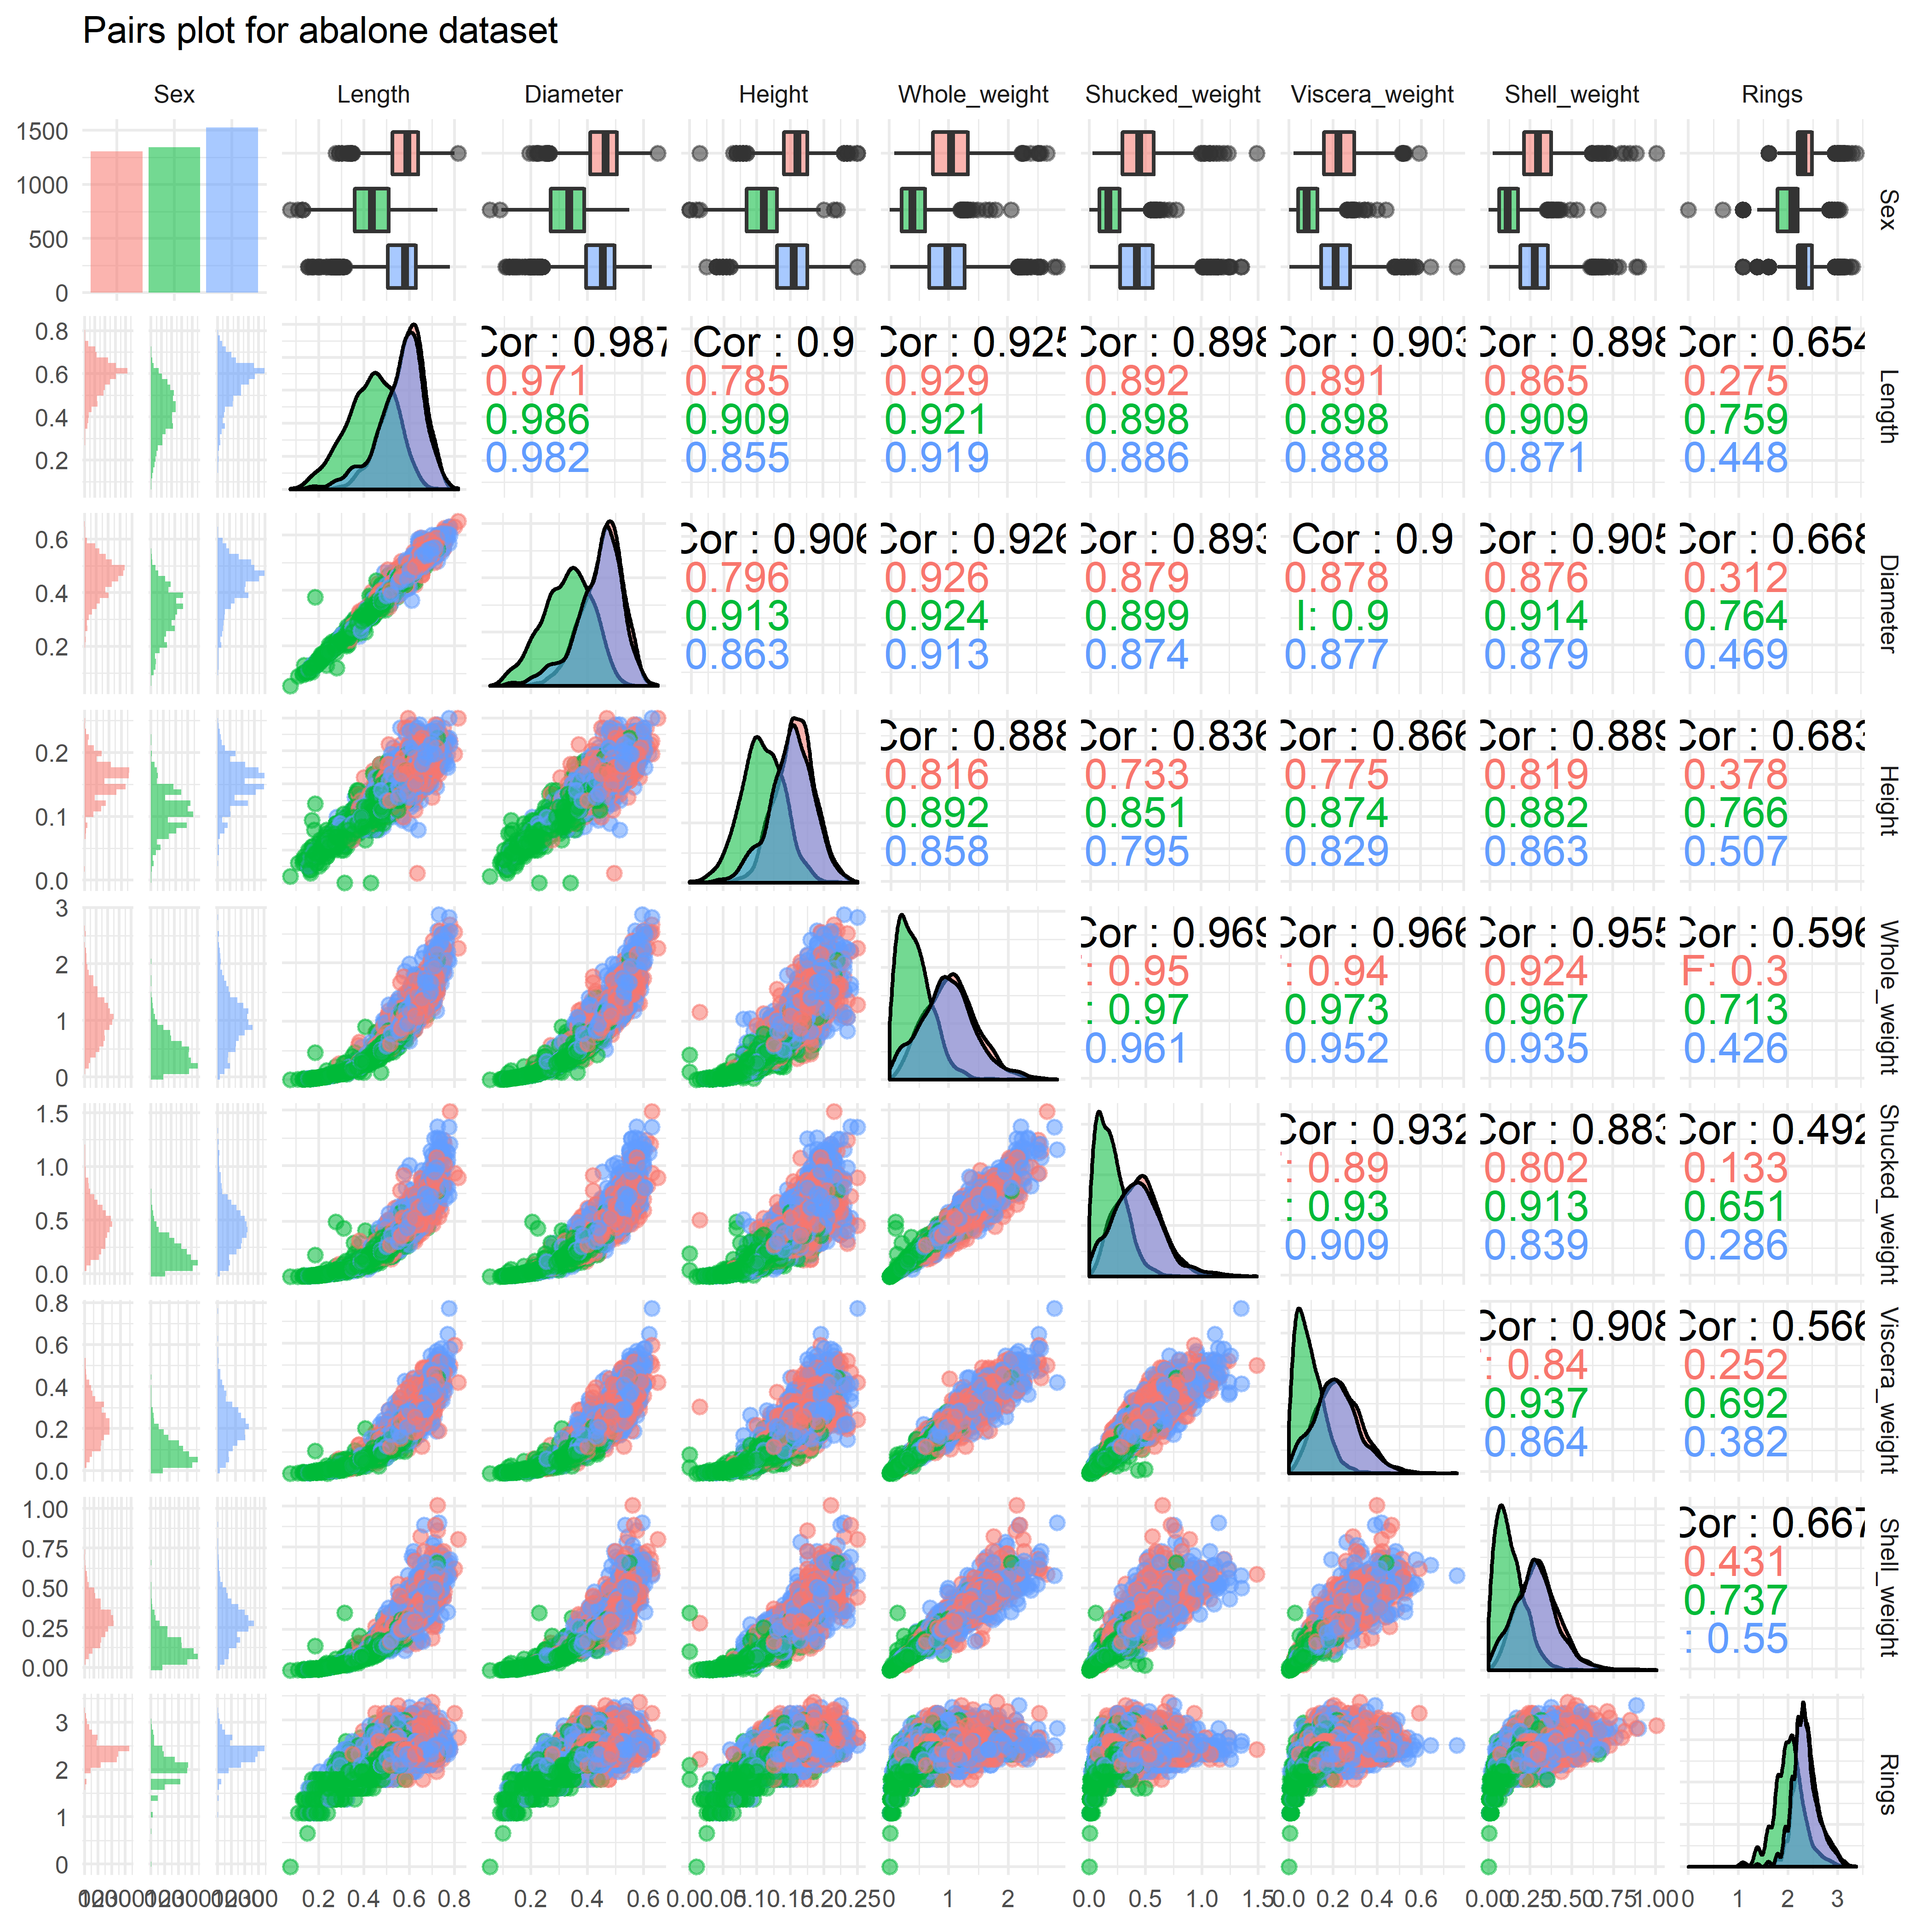
\includegraphics[width=0.85\columnwidth]{ggpairs}
			\caption{GGPairs showing high colinearity}
			\label{fig:ggpairs}
		\end{figure}
		
		
	\section{Analysis}
	The first step is to determine an appropriate model for multiple regression of the data. We use the AIC model selection method in the backwards direction to achieve this. We begin with the full model and remove the least informative variable after every iteration. Crucially, we undergo a log transformation of the dependent variable Rings to ensure normality and homoscedasticity assumptions are held for regression. 
	
	% Please add the following required packages to your document preamble:
	% \usepackage{booktabs}
	\begin{table}[!htbp]
		\centering
		\resizebox{0.3\columnwidth}{!}{%
		\begin{tabular}{@{}ll@{}}
			\toprule
				(Intercept)     & 1.30  \\ \midrule
				SexI            & -0.09 \\
				SexM            & 0.01  \\
				Length          & 0.46  \\
				Diameter        & 1.21  \\
				Height          & 2.63  \\
				Whole\_weight   & 0.60  \\
				Shucked\_weight & -1.61 \\
				Viscera\_weight & -0.90 \\
				Shell\_weight   & 0.49  \\ \bottomrule
				\end{tabular}}
			\caption{Stepback AIC coefficients}
			\vspace{-8mm}
		\label{my-label}
	\end{table}	
	
	The model determined that the following independent variables Sex, Diameter, Height, Shucked\_weight and Viscera\_weight all have a relationship with the log(Rings). Their respective p-values are smaller than the critical value and thus we reject the null hypothesis of no relationship with the log(Rings) variable. Interestingly enough, the degrees of freedom for sex is 2, meaning both infants and males have an effect on the number of rings, but not females. Looking at the qqnorm plot, most of the points are close to the 45 degree line. Hence the normality assumption holds. Furthermore, the residual points are symmetrically distributed above and below the zero line and their spread is fairly constant. Hence the linearity and homoscedasticity assumptions hold as well. Our r-square value is 0.57 which is good as 57\% of the log(Rings) variables can be explained by our constructed model.
	
	\begin{figure}[!htbp]
		\centering
		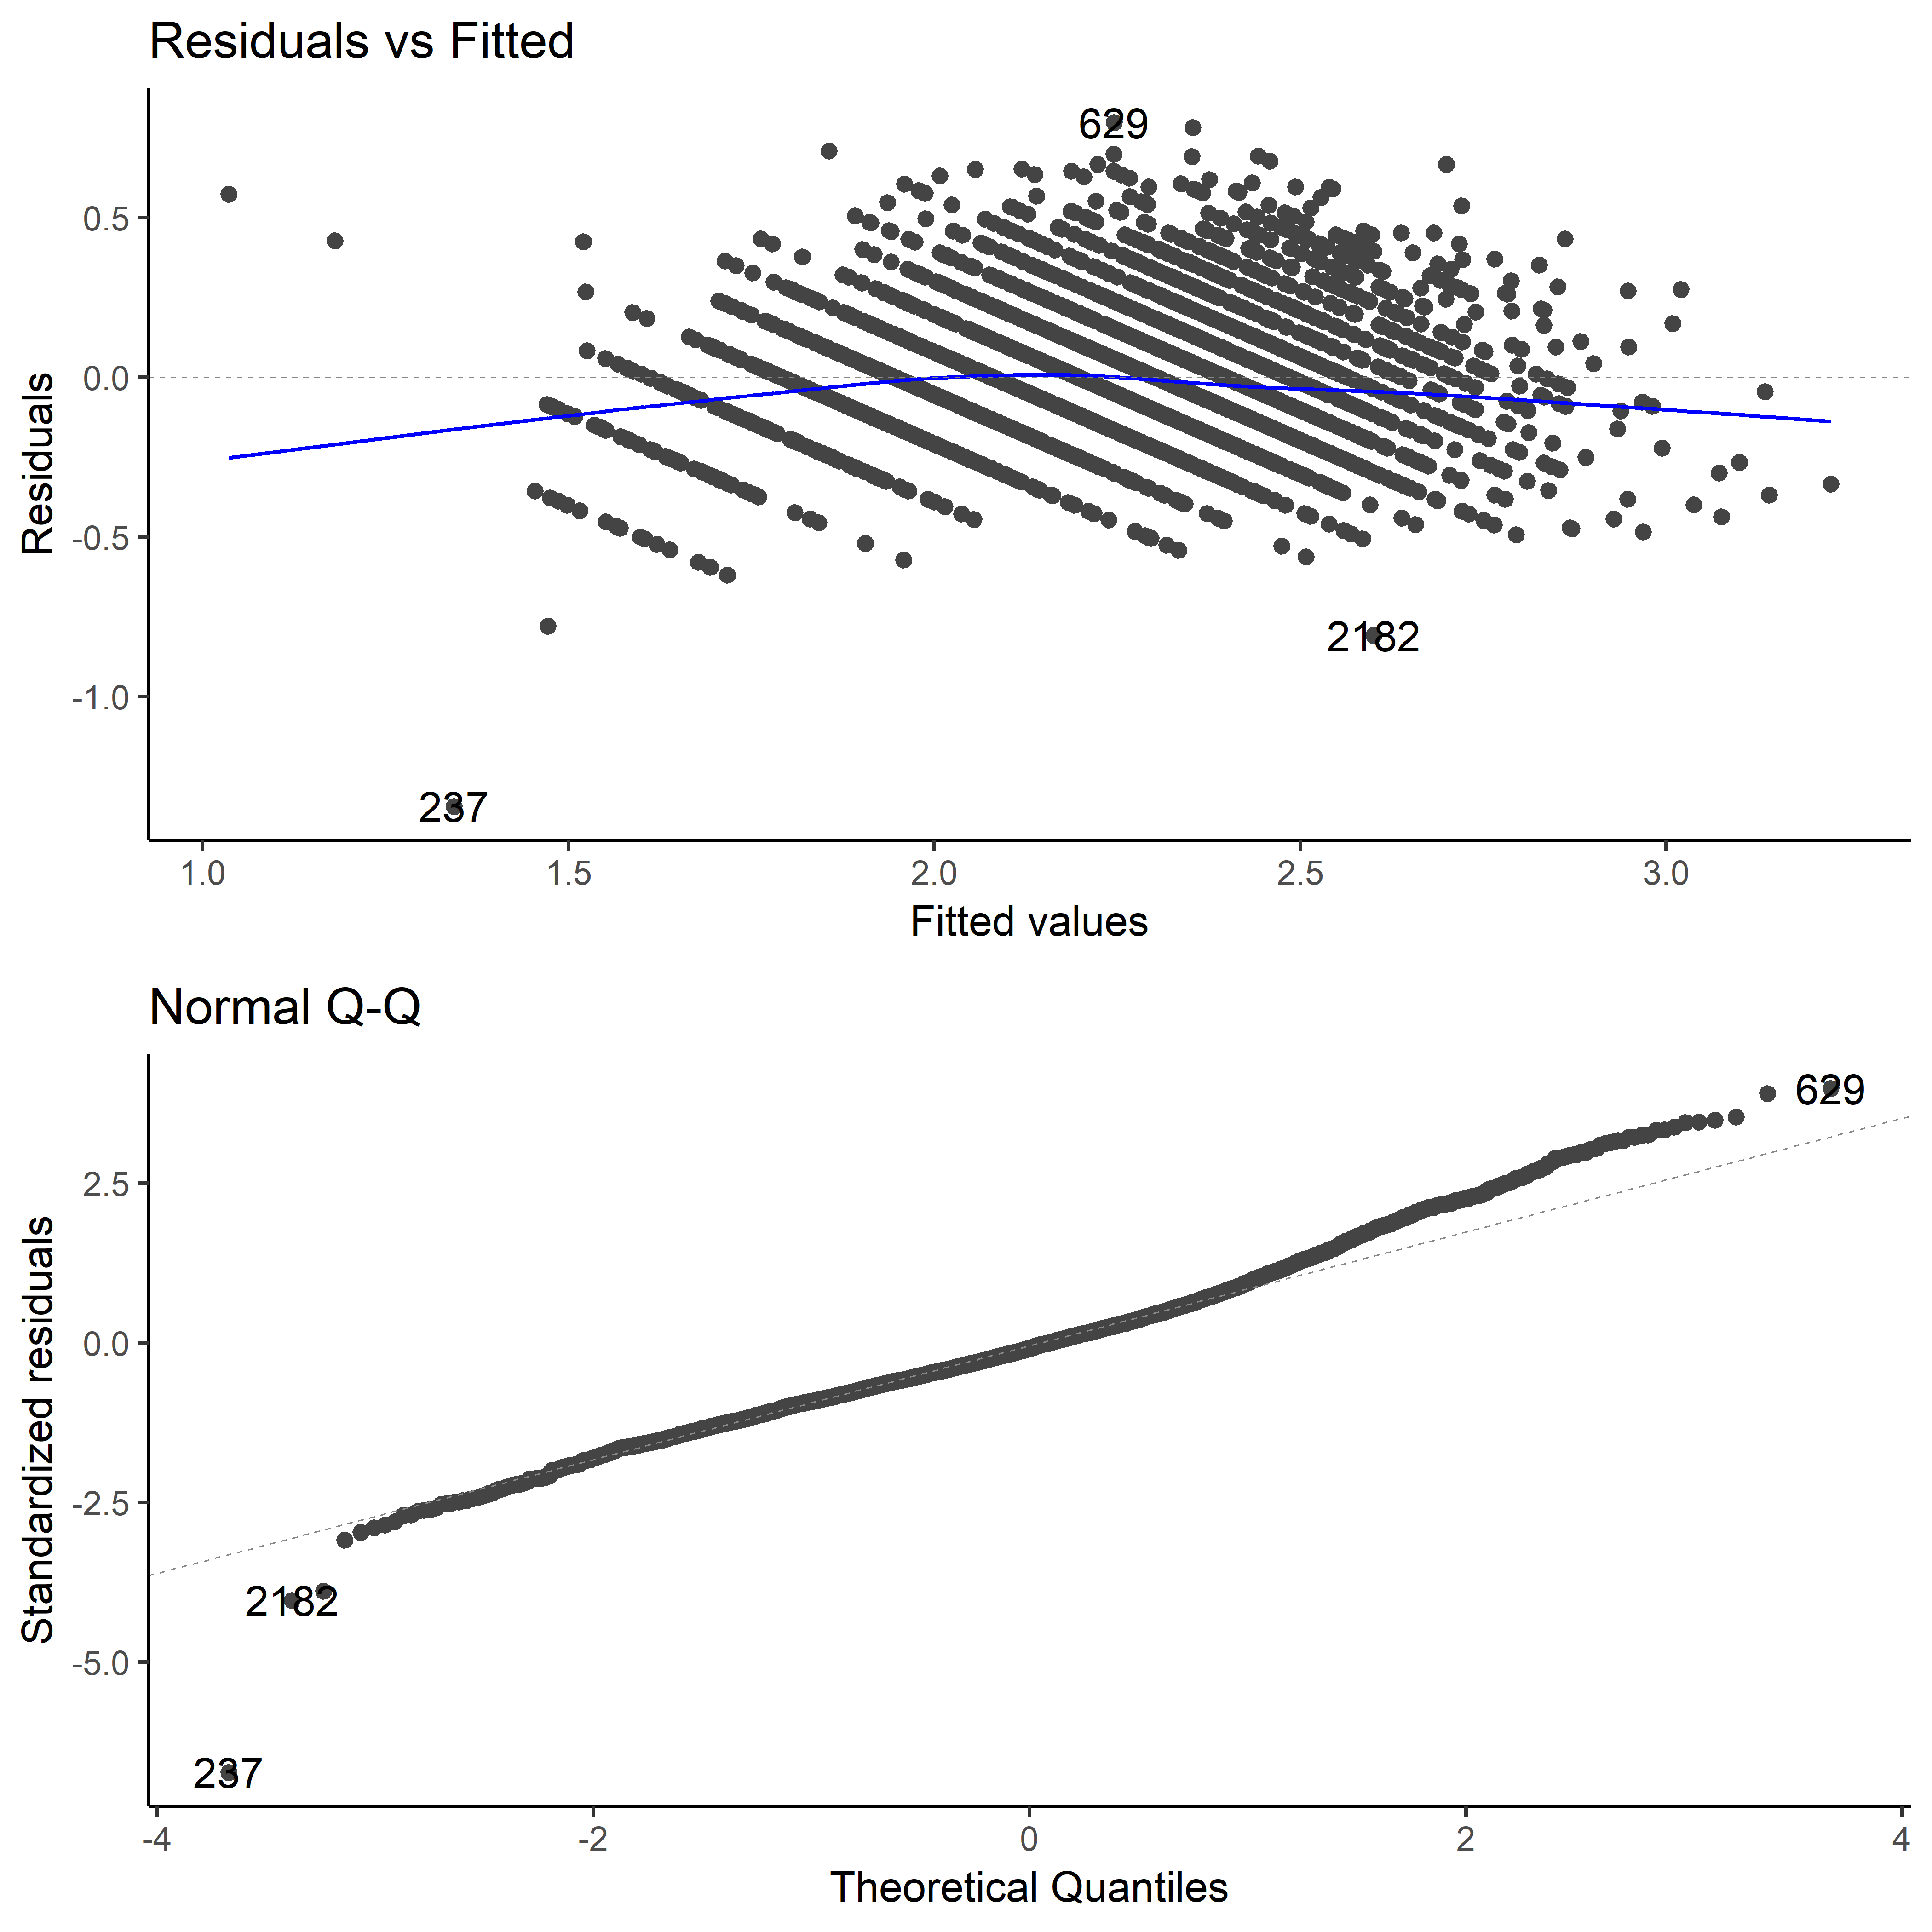
\includegraphics[width=0.7\linewidth]{varnorm}
		\caption{Variance and Normality of Log-Rings}
		\label{fig:varnorm}
	\end{figure}
	\vspace{-8mm}
	
	However, the variables chosen by the model, including Sex, Shucked\_weight and Viscera\_weight can only be determined after cracking open the abalone. This defeats the purpose of the model, as we want to predict as accurate as possible the age of the abalone without opening it to ensure sustainable and efficient farming practices. Thus, a more practical model is chosen with two parameters which are easy to measure without damaging the abalone: weight and diameter. 
	
	As we can see, the r2 value is much higher (0.69 vs 0.57). This suggests that the practical model is a much better fit of the data than the model determined by the AIC method. In addition, it seems as if the normality, linearity and homoscedasticity assumptions all hold as well from looking at the residual and the qqplot. 
	
	
	\section{Results}
	
	\section{Discussion \& Conclusion}
	
	\section{Appendix}
	
	\begin{thebibliography}{9}
		\bibitem{source}
		Abalone. (2018). Dpipwe.tas.gov.au. Retrieved 27 October 2018, from \url{https://dpipwe.tas.gov.au/sea-fishing-aquaculture/community-resources/fish-facts/abalone-blacklip}
		
		\bibitem{blacklip}
		Wild Fisheries Research Program. (2018). Dpi.nsw.gov.au. Retrieved 27 October 2018, from		\url{https://www.dpi.nsw.gov.au/__data/assets/pdf_file/0009/375858/BlacklipAbalone.pdf}
	\end{thebibliography}
\end{document}





























